% !TeX root = ../main.tex

\chapter{评估}
\label{chap:evaluation}

为了测试模型的预测效果,以及利用预测实现的置换和动态参数调节两机制的优化效果,本章将进行半仿真模拟进行评估。评估使用在现实环境中由USRP采集的Wi-Fi流量数据作为背景流量,在此流量的基础上进行数据传输的模拟。Wi-Fi流量的采集在三种环境下进行:
商场(位于一座42层大楼的第3层,总面积约8000平方米),实验室
%\footnote{指在实验室房间内采集的数据,而非Wi-Fi受控的实验室环境。}
(大学校园内,面积约200平方米)和家庭(位于一座7层公寓的第3层,面积约140平方米)中。数据采集的时间从上午10:30到下午9点,一共收集了长度为294小时的Wi-Fi数据。

\section{使用模型进行的预测}
本节从计算复杂度、预测的相关性、准确性和对LDPC解码效果的提升上进行评估。

\textbf{整数分解与蒙特卡罗方法的性能比较}。在第\ref{chap:model}章第\ref{sec:model}节中,我们提到了两种用于进行预测的算法:整数分解和蒙特卡罗方法。图\ref{fig:predict_comparison}对两种算法的性能进行了比较。图\ref{fig:convergence}展示了蒙特卡罗方法的收敛速度,横坐标代表的是每次模拟的随机采样的次数;纵坐标是重复1000次模拟后,每次模拟结果中各个比特位置预测概率的方差的均值。可以看出,蒙特卡罗方法可以很快速的收敛,因此后续模拟中模拟的次数取为100000次。图\ref{fig:complexity}对两个算法的计算次数进行了比较。整数分解的方法在对数图中随着需要预测的帧长度增加而线性增加,说明其增长是指数级别的。一个例子是,在不考率ON/OFF状态的排列下,仅128比特就有4,351,078,600种分解,因此选择蒙特卡罗方法具有更高的效率。
\begin{figure}[b]
	\begin{minipage}[b]{.5\linewidth}
		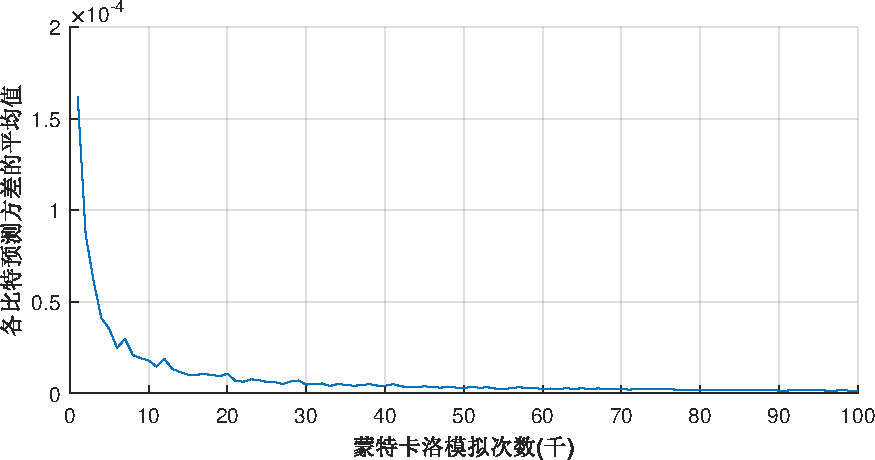
\includegraphics[width = \linewidth]{model_figure2_convergence-cropped}
		\subcaption{蒙特卡洛算法的收敛性。}\label{fig:convergence}
	\end{minipage}
	\hfill
	\begin{minipage}[b]{.5\linewidth}
		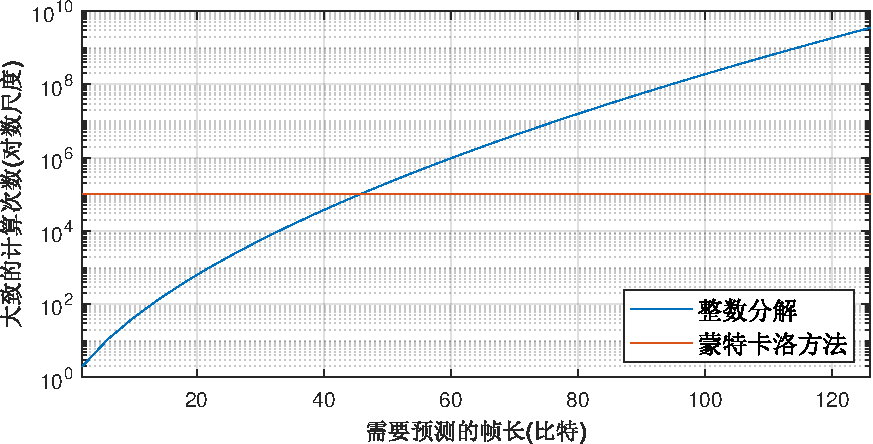
\includegraphics[width = \linewidth]{model_figure3_complexity-cropped}
		\subcaption{对数尺度下两种方法计算次数比较。}\label{fig:complexity}
	\end{minipage}
	\caption{整数分解与蒙特卡罗方法的性能比较。}\label{fig:predict_comparison}
\end{figure}

\textbf{预测的相关性}。在第\ref{sec:model}节中提到Wi-Fi流量具有一定的持续性;直观上,如果两个相邻时间段的ON/OFF经验累积分布函数是相似的话,可以用前一时段的统计结果对后一时段的数据进行预测。具体实现中,给定两个时间段$\Delta_i = [t_i, t_{i+1}]$和$\Delta_{i+1} = [t_{i+1}, t_{i+2}]$。在$\Delta_i$内来利用统计的累积分布函数$F_{ON},F_{OFF}$生成长度为$w$的窗口的模拟流量,用来与$\Delta_{i+1}$随机采样得到的长度同为$w$的实际流量进行柯尔莫哥洛夫-斯米尔诺夫检验(KS检验)来判断相关性。如果有$n$个窗口,假设有$0.95n$个窗口中KS检验接受了零假设,那么便可以以95\%的置信度认为两个时间段的分布是相似的。

图\ref{fig:kstest}对使用相邻时间段内的统计数据进行预测的可靠程度进行了分析,时间段的划分为10分钟,窗口大小$w$为100毫秒,测试次数为1000个窗口。横轴代表测试的环境参数,纵轴代表KS检验的通过率,红色与蓝色的点分别表示对ON状态的检验和对OFF状态的检验,在同一横坐标下的不同点代表了不同的两个相邻时间段测试的通过率。在商场和家庭中,OFF状态存在较高的相关度,但ON状态的相关度较低;在实验室环境下,不论是ON状态还是OFF状态都存在很高的相关度,平均通过率在96.7\%和97.1\%。这说明,在中等人数且比较稳定的环境(比如实验室)下,使用环境中的Wi-Fi数据有很好的相关性;在人数变化或比较少的情况下,相关性会有所下降。
\begin{figure}[t]
	\centering
	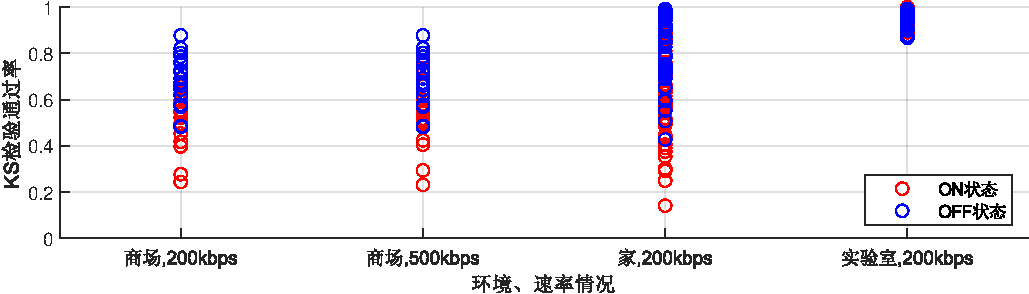
\includegraphics[width = \linewidth]{eval_figure1_sliding-cropped}
	\caption{相邻两时间窗口KS检验的通过率。}
	\label{fig:kstest}
\end{figure}

\textbf{预测的准确性}。相关性在一方面评估了模型的可靠性,但受限于窗口$w$的大小并不能完整展示出模型预测的效果。一方面,过大的窗口会远离模型希望实现短时段内预测的目标;另一方面,过小的窗口不能收集足够的数据用于进行KS检验。准确性检验了模型预测与实际发送中遇到的ON/OFF状态的符合程度,具体来讲是计算每一比特上的估计与正确状态一致(击中)的比例,即击中率。首先,在当前时间段内依据模型计算对下一时间段的预测;在指定阈值后(见第\ref{subsec:perm}段),预测概率值大于阈值的部分认为是ON,否则是OFF。然后再从下一时间段中随机采样到实际传输中的ON/OFF状态,将预测与真实状态按每一位进行比较,计算击中的比例,越高说明预测越准确。

图\ref{fig:hitmap}展示了击中率的热力图,从下一时间段采样的次数为1000次。与相关性分析比较相近的是,实验室环境的预测很准确,图\ref{fig:hitmap_256_500_0.6_lab}中平均击中率达到了98.6\%;但商场和家庭环境的预测击中率稍低,图\ref{fig:hitmap_256_500_0.6_mall}和\subref{fig:hitmap_256_500_0.6_home}的平均击中率在84.7\%和67.5\%。同时,越高的速率和越短的帧长击中率越高,这也与相关性分析比较一致。值得注意的是,阈值设置的比0.5稍高一些可以提升预测的效果,参照图\ref{fig:hitmap_256_500_0.6_mall}和图\subref{fig:hitmap_256_500_0.5_mall}展示的结果,两图中平均的击中率分别是84.24\%和79.06\%。这可能来源于预测从ON状态开始,因此会更加偏向预测当前状态为ON,更高的阈值可以平衡掉这种偏好。
\begin{figure}[t]
	\begin{minipage}[b]{.32\linewidth}
		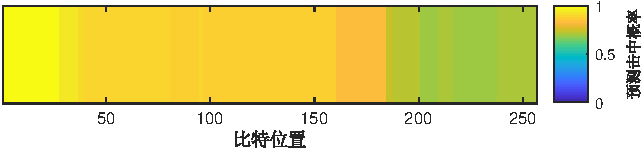
\includegraphics[width = \linewidth]{eval_figure2_1_256_500_mall-cropped}
		\subcaption{商场环境,256比特,500kbps,阈值0.6。}\label{fig:hitmap_256_500_0.6_mall}
	\end{minipage}
	\hfill
	\begin{minipage}[b]{.32\linewidth}
		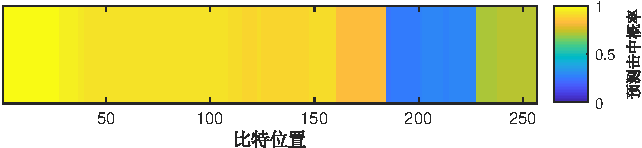
\includegraphics[width = \linewidth]{eval_figure2_2_256_500_mall-cropped}
		\subcaption{商场环境,256比特,500kbps,阈值0.5。}\label{fig:hitmap_256_500_0.5_mall}
	\end{minipage}
	\hfill
	\begin{minipage}[b]{.32\linewidth}
		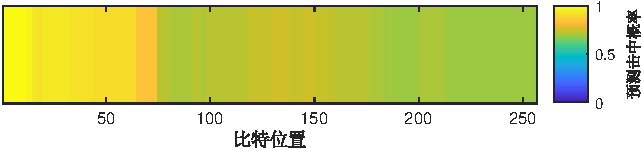
\includegraphics[width = \linewidth]{eval_figure2_1_256_200_mall-cropped}
		\subcaption{商场环境,256比特,200kbps,阈值0.6。}\label{fig:hitmap_256_200_0.6_mall}
	\end{minipage}
	
	\begin{minipage}[b]{.32\linewidth}
		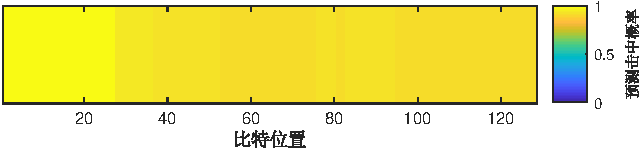
\includegraphics[width = \linewidth]{eval_figure2_1_128_500_mall-cropped}
		\subcaption{商场环境,128比特,500kbps,阈值0.6。}\label{fig:hitmap_128_500_0.6_mall}
	\end{minipage}
	\hfill
	\begin{minipage}[b]{.32\linewidth}
		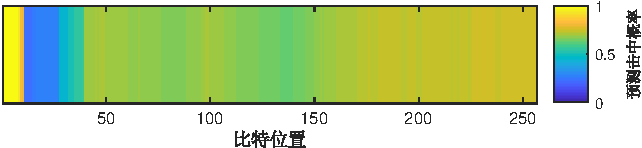
\includegraphics[width = \linewidth]{eval_figure2_1_256_500_home-cropped}
		\subcaption{家庭环境,256比特,500kbps,阈值0.6。}\label{fig:hitmap_256_500_0.6_home}
	\end{minipage}
	\hfill
	\begin{minipage}[b]{.32\linewidth}
		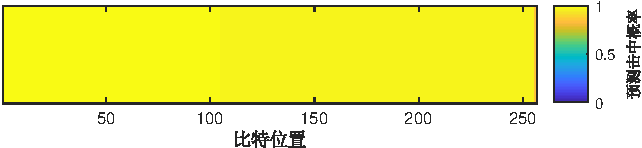
\includegraphics[width = \linewidth]{eval_figure2_1_256_500_lab-cropped}
		\subcaption{实验室环境,256比特,500kbps,阈值0.6。}\label{fig:hitmap_256_500_0.6_lab}
	\end{minipage}
	\caption{不同环境、不同帧长、不同传输速率下的预测击中热力图。}\label{fig:hitmap}
\end{figure}

\textbf{预测对LDPC解码效果的提升}。在结合预测情况下可以以此为信道先验实施LDPC解码。图\ref{fig:ldpc}展示了在商场环境下不同帧长、不同传输速率的使用LDPC码的比特错误率。使用的编码是$(96,48)$,列权重为$3$的规则LDPC码\footnote{校验矩阵来自http://www.inference.org.uk/mackay/CodesFiles.html.}。可以看到,不论帧长和码率是何种情况,结合信道情况的解码都比无信道情况的解码有显著的提升,图\ref{fig:ldpc_256_200}中,在SNR=14dB的情况下,预测的LDPC使得BER下降了99.8\%。蓝线是完全知道ON/OFF的具体位置情况下的LDPC解码效果,即全知情况。尽管使用预测信息的解码表现有一定差距,但是整体上还是比较接近的。
\begin{figure}[t]
	\begin{minipage}[b]{.32\linewidth}
		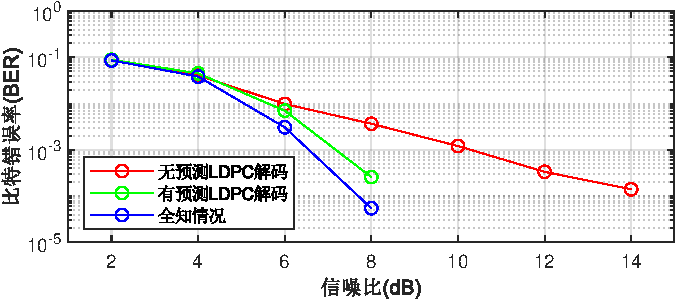
\includegraphics[width = \linewidth]{eval_figure3_LDPC_128_500_mall-cropped}
		\subcaption{商场环境,128比特,500kbps。}\label{fig:ldpc_128_500}
	\end{minipage}
	\hfill
	\begin{minipage}[b]{.32\linewidth}
		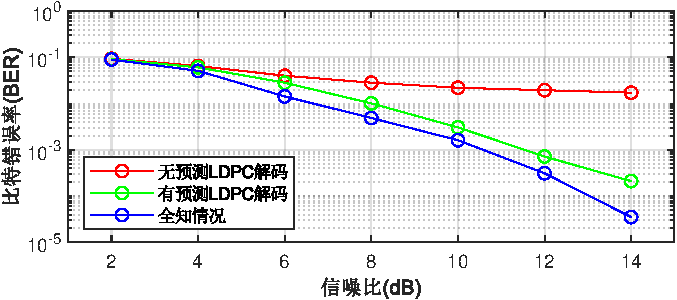
\includegraphics[width = \linewidth]{eval_figure3_LDPC_256_200_mall-cropped}
		\subcaption{商场环境,256比特,200kbps。}\label{fig:ldpc_256_200}
	\end{minipage}
	\hfill
	\begin{minipage}[b]{.32\linewidth}
		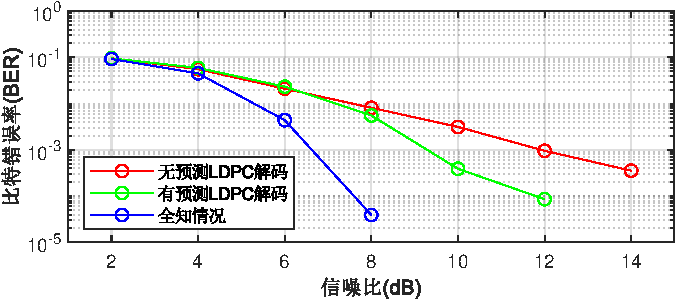
\includegraphics[width = \linewidth]{eval_figure3_LDPC_256_500_mall-cropped}
		\subcaption{商场环境,256比特,500kbps。}\label{fig:ldpc_256_500}
	\end{minipage}
	\caption{预测对LDPC解码效果的提升。}\label{fig:ldpc}
\end{figure}

\begin{figure}[t]
	\begin{minipage}[b]{.32\linewidth}
		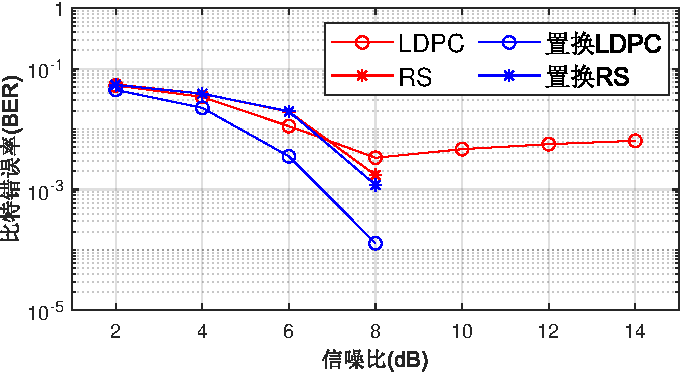
\includegraphics[width = \linewidth]{eval_figure4_allTogethrt_256_500_mall-cropped}
		\subcaption{商场下,500kbps。}\label{fig:ber_500_mall}
	\end{minipage}
	\hfill
	\begin{minipage}[b]{.32\linewidth}
		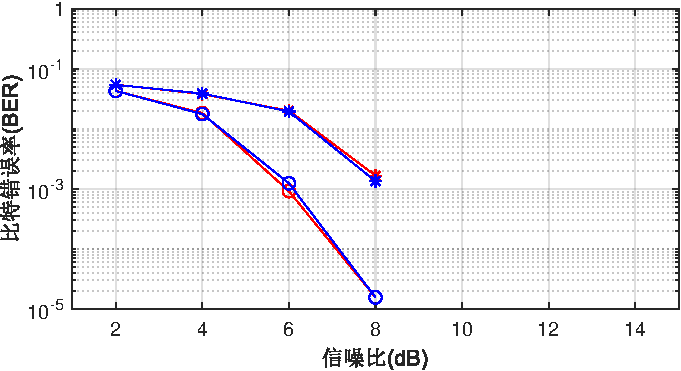
\includegraphics[width = \linewidth]{eval_figure4_allTogethrt_256_500_lab-cropped}
		\subcaption{实验室下,500kbps。}\label{fig:ber_500_lab}
	\end{minipage}
	\hfill
	\begin{minipage}[b]{.32\linewidth}
		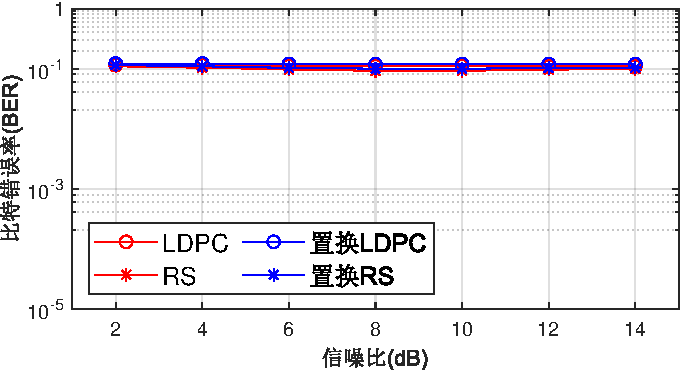
\includegraphics[width = \linewidth]{eval_figure4_allTogethrt_256_500_home-cropped}
		\subcaption{家庭下,500kbps。}\label{fig:ber_500_home}
	\end{minipage}
	
	\begin{minipage}[b]{.32\linewidth}
		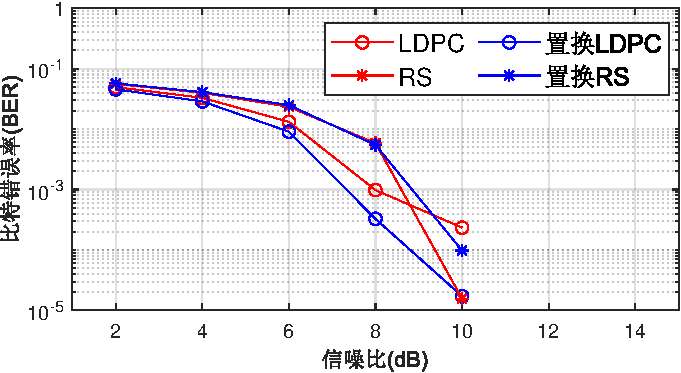
\includegraphics[width = \linewidth]{eval_figure4_allTogethrt_256_200_mall-cropped}
		\subcaption{商场下,200kbps。}\label{fig:ber_200_mall}
	\end{minipage}
	\hfill
	\begin{minipage}[b]{.32\linewidth}
		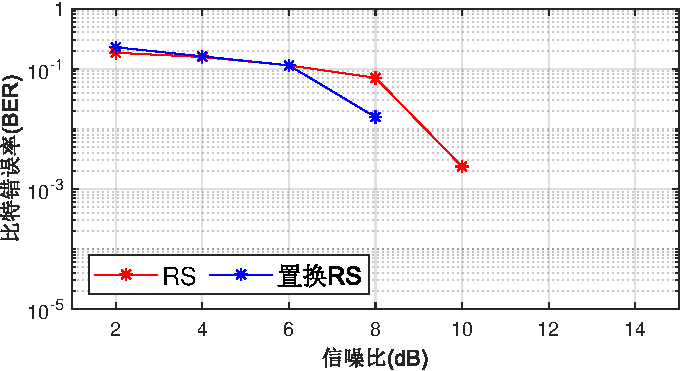
\includegraphics[width = \linewidth]{eval_figure4_RS27_256_500_lab-cropped}
		\subcaption{图\subref{fig:ber_500_lab}相同条件,码率升高。}\label{fig:ber_500_lab_cr}
	\end{minipage}
	\hfill
	\begin{minipage}[b]{.32\linewidth}
		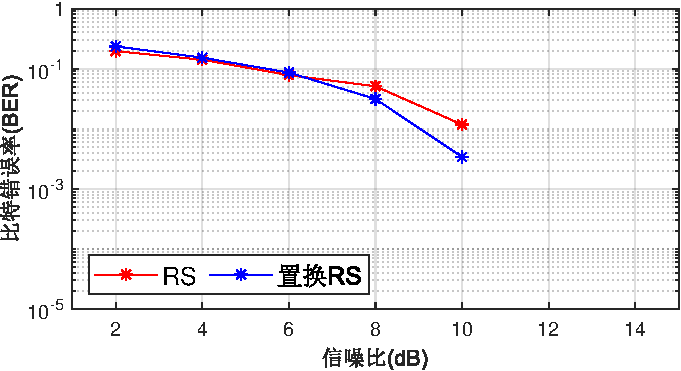
\includegraphics[width = \linewidth]{eval_figure4_RS27_256_200_home-cropped}
		\subcaption{图\subref{fig:ber_500_home}相同条件,码率降低。}\label{fig:ber_500_home_cr}
	\end{minipage}
	
	\begin{minipage}[b]{.32\linewidth}
		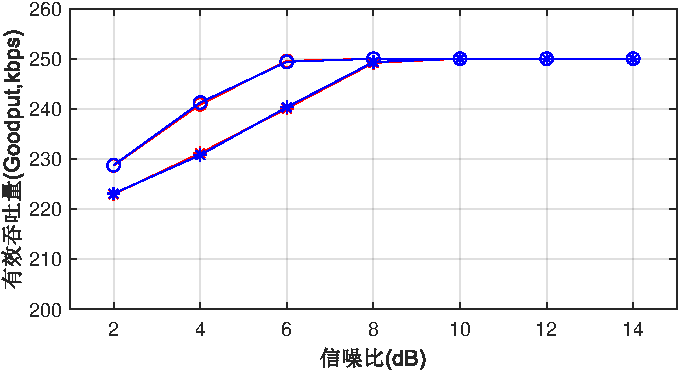
\includegraphics[width = \linewidth]{eval_figure4_goodput_256_500_lab-cropped}
		\subcaption{实验室下,500kbps。}\label{fig:goodput_500_lab}
	\end{minipage}
	\hfill
	\begin{minipage}[b]{.32\linewidth}
		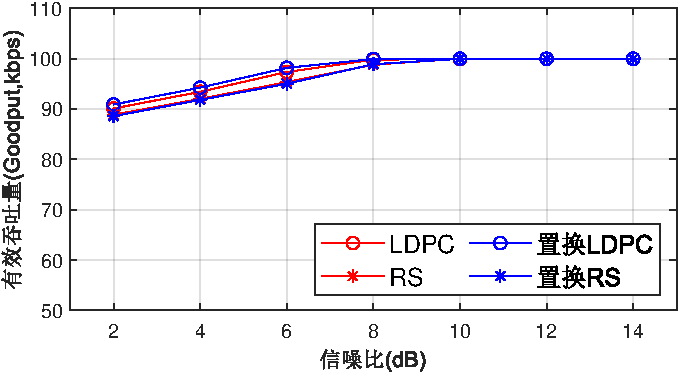
\includegraphics[width = \linewidth]{eval_figure4_goodput_256_200_mall-cropped}
		\subcaption{商场下,200kbps。}\label{fig:goodput_200_lab}
	\end{minipage}
	\hfill
	\begin{minipage}[b]{.32\linewidth}
		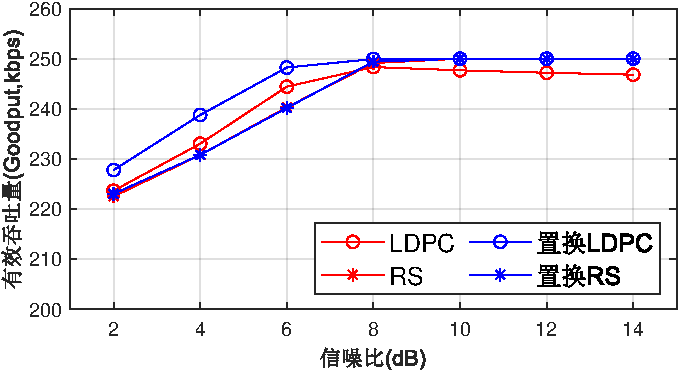
\includegraphics[width = \linewidth]{eval_figure4_goodput_256_500_mall-cropped}
		\subcaption{商场下,500kbps。}\label{fig:goodput_500_mall}
	\end{minipage}
	
	\caption{LDPC、置换LDPC、RS、置换RS比特错误率和有效吞吐量比较(帧长为256比特)。}\label{fig:ber}
\end{figure}
\section{使用模型进行的优化}

\textbf{置换对LDPC和RS码的性能提升}。图\ref{fig:ber}展示了在三种环境下,使用不同速率和编码方式的比特错误率和有效传输率表现。其中,LDPC码使用的是$(96,48)$,列权重为$3$的规则LDPC码;RS为$(31,15)$的编码,有效传输率由单位时间内被正确传输的比特计算。两种编码的码率相近,同时总长度、信息长度也相近,因此可以做一定的比较。

\begin{enumerate}
	\item LDPC码与RS码的比较。总体来看,LDPC的表现优于RS。
	图\ref{fig:ber_500_home}由于环境中Wi-Fi流量过于稀少,超出了编码的恢复能力,因此呈现平直的线。虽然LDPC的效果更好,但是这是在牺牲运算速度的情况下;通常RS编码有专用的硬件进行加速。因此采用LDPC码可能会使的实际使用中的传输速度有所下降,同时能耗也可能更高。
	
	\item 置换与不置换的比较。在高信噪比的情况下,置换与不置换的效果差别不大,这是由于高信噪比下噪声更影响解码的效果,信道的“归零”效果不如噪声显著。图\ref{fig:ber_500_mall}和\subref{fig:ber_200_mall}中置换与不置换的差别相比更明显。在商场环境下置换使LDPC码的比特错误率有所下降。但对于RS码,置换的效果有限,这可能是由RS不依靠信道先验概率影响,只考虑错误发生的位置,使得置换前后影响的码元数没有大的变化;而LDPC在置换后原有不受影响的块受到了OFF状态的影响,且受先验概率的不准确导致这些不受影响的块在使用信念传播算法的过程中错误率提升,导致最终总体看来比特错误有下降。
	
	而在实验室和家庭环境下,由于OFF状态很少或很多,使得置换与不置换的效果相近。因此图\ref{fig:ber_500_lab_cr}和\subref{fig:ber_500_home_cr}对RS码的码率进行了相应的升高和降低。可以看出,置换对RS码的表现是有提升的。
	
	\item 有效吞吐率。在有效吞吐率方面,在高信噪比的情况下几乎都可以有效的传输数据,而在较低信噪比下与各个编码在对应环境下的比特错误率表现也是一致的。相差最大的情况下(实验室,500kbps,SNR=4dB),LDPC相比RS实现了5\%的提升(11kbps)。
\end{enumerate}

\begin{figure}[t]
	\begin{minipage}[b]{.32\linewidth}
		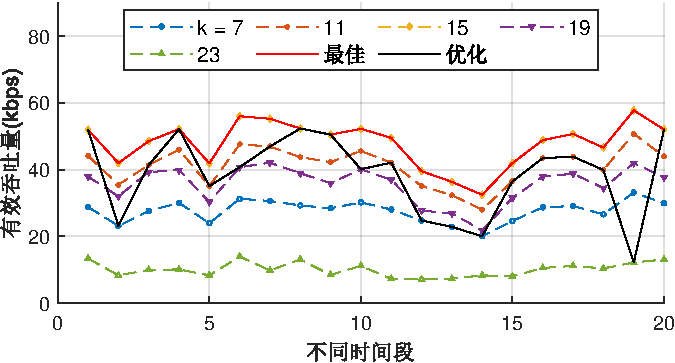
\includegraphics[width = \linewidth]{eval_figure5_optCodeRate_256_200_mall_8-cropped}
		\subcaption{商场环境,256比特,200kbps。}\label{fig:coderate_256_200_mall}
	\end{minipage}
	\hfill
	\begin{minipage}[b]{.32\linewidth}
		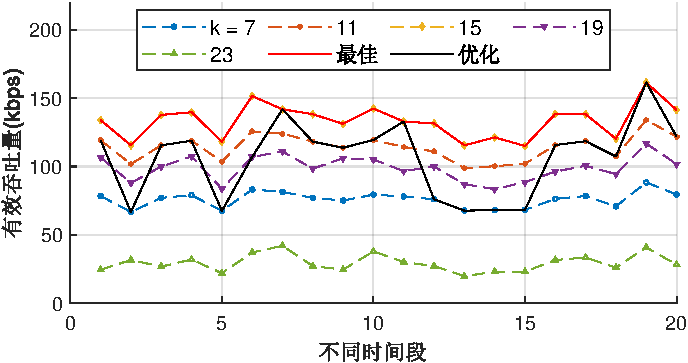
\includegraphics[width = \linewidth]{eval_figure5_optCodeRate_256_500_mall_8-cropped}
		\subcaption{商场环境,256比特,500kbps。}\label{fig:coderate_256_500_mall}
	\end{minipage}
	\hfill
	\begin{minipage}[b]{.32\linewidth}
		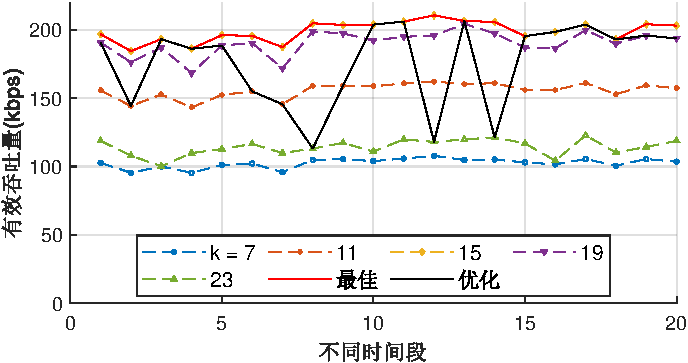
\includegraphics[width = \linewidth]{eval_figure5_optCodeRate_128_500_mall_8-cropped}
		\subcaption{商场环境,128比特,500kbps。}\label{fig:coderate_128_500_mall}
	\end{minipage}

	\begin{minipage}[b]{.32\linewidth}
		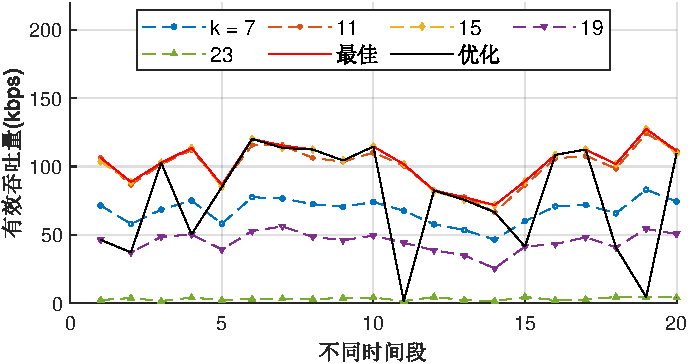
\includegraphics[width = \linewidth]{eval_figure5_optCodeRate_512_500_mall_8-cropped}
		\subcaption{商场环境,512比特,500kbps。}\label{fig:coderate_512_500_mall}
	\end{minipage}
	\hfill
	\begin{minipage}[b]{.32\linewidth}
		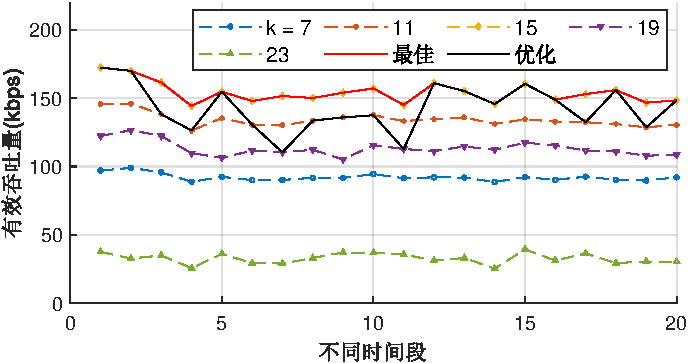
\includegraphics[width = \linewidth]{eval_figure5_optCodeRate_256_500_lab_8-cropped}
		\subcaption{实验室环境,256比特,500kbps。}\label{fig:coderate_256_200_lab}
	\end{minipage}
	\hfill
	\begin{minipage}[b]{.32\linewidth}
		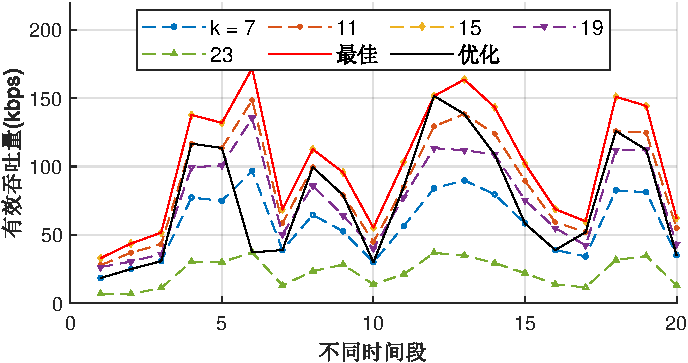
\includegraphics[width = \linewidth]{eval_figure5_optCodeRate_256_500_home_8-cropped}
		\subcaption{家庭环境,256比特,500kbps。}\label{fig:coderate_256_200_home}
	\end{minipage}
	\caption{不同环境下动态调节码率对实际吞吐量的影响。}\label{fig:coderate}
\end{figure}
\textbf{对RS码的动态参数调节}。
图\ref{fig:coderate}展示了在不同环境、速率和帧长下,利用模型的预测结果对RS码码率调节的效果。这里采用的是$(31, k)$的RS码。横坐标表示不同的时间段,纵坐标表示有效吞吐量。在商场环境下,不同帧长和速率会有不同的ON/OFF统计特征,这也表现在图中$k$值从上到下的顺序会发生改变。图\ref{fig:coderate_256_200_mall}-\subref{fig:coderate_128_500_mall}中,在$k = 15$都达到了最高的有效吞吐量,在错误恢复和传输信息之间取得了平衡。从结果来看,预测的效果能够以平均65\%的概率击中最好的两个码率;在没有选择最佳两个码率的情况下,多数选择了高码率的情况。这可能来源于对长度的平衡不够合理。总体来看,在商场环境下使用预测优化的码率能够达到最佳吞吐量的80.79\%,最好的情况下达到88.25\%。

对比商场、实验室和家庭三种环境下的有效吞吐量,我们可以发现:
\begin{enumerate}
	\item 基于预测选择的码率的最优两个码率的击中率与ON/OFF状态预测的击中率正相关。实验室环境下状态预测更准确,因此最优两个码率的击中率能达到80\%,高于商场的65\%;而家庭环境中状态预测不够准确,因此最优两个码率的击中率仅为45\%。
	
	\item 基于预测选择的码率随着环境中ON/OFF统计特征的变化而变化。这在图\ref{fig:coderate_256_200_home}中表现最为明显:家庭下的ON/OFF状态变化比较剧烈,最优码率呈现上下起伏的变化,而预测给出的码率(图中黑线)也伴随着这种趋势选择不同的码率。
	
	\item 在实验室条件(图\ref{fig:coderate_256_200_lab})下,使用预测优化的码率能够达到最佳吞吐量的89.63\%;而在家庭条件
	(图\ref{fig:coderate_256_200_home})下能达到65.85\%。
\end{enumerate}
